\documentclass[11pt,a4paper]{article}

% -----------------------------------------------------------------------------
% Paquetes: todos forman parte de una instalación estándar de LaTeX.
% -----------------------------------------------------------------------------
\usepackage[utf8]{inputenc}
\usepackage[T1]{fontenc}
% Fecha en español sin depender de babel ni de spanish.ldf.
\newcommand{\FechaEnEspanol}{%
  \number\day\space de\space
  \ifcase\month
    \or enero\or febrero\or marzo\or abril\or mayo\or junio\or
    julio\or agosto\or septiembre\or octubre\or noviembre\or diciembre
  \fi\space de\space\number\year
}
\usepackage[a4paper,margin=2.5cm,headheight=42pt]{geometry}
\usepackage{graphicx}
\usepackage{tikz}
\usepackage{xcolor}
\usepackage{fancyhdr}
\usepackage[hidelinks]{hyperref}
\hypersetup{pdftitle={teorico-tp-1}}

% lastpage no es necesario para compilar, pero permite mostrar "página de N".
\newif\ifHayUltimaPagina
\IfFileExists{lastpage.sty}{
  \usepackage{lastpage}
  \HayUltimaPaginatrue
}{
  \HayUltimaPaginafalse
}

% -----------------------------------------------------------------------------
% CONFIGURACIÓN DEL TRABAJO: editar solamente este bloque para reutilizarlo.
% -----------------------------------------------------------------------------
\newcommand{\NombreMateria}{Redes de Computadoras}
\newcommand{\TipoTrabajo}{Trabajo Práctico}
\newcommand{\NumeroTrabajo}{1}
% Cambiar por "Teórico" o "Práctico" según corresponda.
\newcommand{\TipoTP}{Teórico}
\newcommand{\NombreTrabajo}{Introducción a los Sistemas de Comunicaciones}
\newcommand{\NombreGrupo}{NetRunners}
\newcommand{\Docente}{FACUNDO NICOLAS OLIVA CUNEO}
\newcommand{\LogoArchivo}{logo.png}
\newcommand{\LogoRuta}{\LogoArchivo}

% Una línea por integrante. Se pueden agregar o quitar filas.
\newcommand{\Integrantes}{%
  \begin{tabular}{ll}
    Bastida, Lucas Ramiro & DNI 39444511 \\
    Contessi, Ruben Andres & DNI 33315235 \\
    Garay, Ignacio Hernan & DNI 44191925 \\
    Giraudo, Juan Pablo & DNI 34970089 \\
    Peñaloza, Gonzalo Adrian & DNI 40441355 \\
    Quinteros del Castillo, Tomás Agustín & DNI 46169739 \\
    Vasconsellos Blason, Benjamin Alejandro & DNI 45642879 \\
  \end{tabular}%
}

% -----------------------------------------------------------------------------
% Elementos comunes de carátula y encabezado.
% -----------------------------------------------------------------------------
\newcommand{\InsertarLogo}[1][0.24\textwidth]{%
  \ifx\LogoRuta\empty
    \fbox{\parbox[c][1cm][c]{#1}{\centering Logo institucional\\\small (colocar archivo)}}%
  \else
    \includegraphics[width=#1,keepaspectratio]{\LogoRuta}%
  \fi
}

\newcommand{\TituloCorto}{TP \NumeroTrabajo (\TipoTP): \NombreTrabajo}

% Eje temporal normalizado: una unidad horizontal representa un período T.
\newcommand{\EjeTiempo}[1]{%
  \draw[->] (-1.15,0) -- (1.25,0) node[right] {\small Tiempo};
  \draw[->] (0,-#1) -- (0,#1) node[above] {\small Amplitud};
  \foreach \x/\etiqueta in {-1/-T,-0.5/{-\frac{T}{2}},0.5/{\frac{T}{2}},1/T} {
    \draw (\x,0.10) -- (\x,-0.10) node[below=2pt] {\scriptsize $\etiqueta$};
  }
}

\pagestyle{fancy}
\fancyhf{}
\fancyhead[L]{\InsertarLogo[1.4cm]}
\fancyhead[C]{\small\textbf{\TituloCorto}}
\fancyhead[R]{\small\NombreGrupo}
\renewcommand{\headrulewidth}{0.4pt}
\fancyfoot[C]{\small Página \thepage\ifHayUltimaPagina\ de \pageref{LastPage}\fi}
\renewcommand{\footrulewidth}{0pt}

\begin{document}

\begin{titlepage}
  \thispagestyle{empty}
  \begin{center}
    \InsertarLogo[0.32\textwidth]

    \vfill
    {\Large\textsc{\NombreMateria}\par}
    \vspace{1.5cm}
    {\Huge\bfseries \TipoTrabajo\par}
    \vspace{0.35cm}
    {\LARGE N.\textsuperscript{o} \NumeroTrabajo (\TipoTP)\par}
    \vspace{0.8cm}
    {\Large\NombreTrabajo\par}

    \vfill
    \begin{tabular}{rl}
      \textbf{Grupo:} & \NombreGrupo \\
      \textbf{Docente:} & \Docente
    \end{tabular}

    \vspace{1cm}
    \begin{center}
      \textbf{Integrantes}\\[0.2cm]
      \Integrantes
    \end{center}

    \vfill
    {\large \FechaEnEspanol\par}
  \end{center}
\end{titlepage}

\section*{b) - Preguntas:}

\noindent\textbf{3.1}\par
En un medio guiado las ondas electromagnéticas que se usan para transmitir los datos se propagan confinadas en un camino físico o material, por ejemplo, cables metálicos o fibras ópticas. Es direccional: la información llegará allá donde llegue el material físico, por lo que este debe conectarse entre emisor y receptor para que la comunicación pueda realizarse.

En un medio no guiado la transmisión de las ondas se produce irradiándolas en un medio, manipulando el campo electromagnético. Su propagación se produce en múltiples direcciones (aunque pudiendo lograr cierta direccionalidad mediante diseños específicos de transmisores). Esto permite al receptor estar en cualquier punto dentro del radio de potencia de transmisión del emisor e incluso que ambos actores puedan estar en movimiento.

\noindent\textbf{3.2}\par\vspace{\baselineskip}
\noindent\textbf{3.3}\par\vspace{\baselineskip}
\noindent\textbf{3.4}\par\vspace{\baselineskip}
\noindent\textbf{3.5}\par\vspace{\baselineskip}
\noindent\textbf{3.6}\par\vspace{\baselineskip}
\noindent\textbf{3.7}\par
La atenuación es la pérdida progresiva de energía o potencia que sufre una señal a medida que viaja a través de un medio de transmisión. Ocurre tanto por un aumento de la distancia entre emisor y receptor como por un incremento de la frecuencia de la señal. Por lo tanto, puede ser necesario el uso de amplificadores o repetidores para recuperar la potencia y de ecualizadores para corregir la distorsión por frecuencia. 
\noindent\textbf{3.8}\par

Se denomina capacidad del canal a la velocidad máxima a la que se pueden transmitir los datos en un canal, o ruta de comunicación de datos, bajo unas condiciones dadas, expresada en bits por segundo (bps).

\noindent\textbf{3.9}\par\vspace{\baselineskip}

\section*{c)- Ejercicios:}

\noindent\textbf{3.1}\par
\noindent a). En una configuración multipunto múltiples dispositivos comparten el mismo medio de transmisión, por lo que si más de uno transmite al mismo tiempo, las señales se solaparían y los mensajes serían indistinguibles.\par
\noindent b).  \par
\begin{center}
  \begin{tabular}{|l|p{0.32\textwidth}|p{0.32\textwidth}|}
    \hline
    & \textbf{Centralizado} & \textbf{Descentralizado} \\
    \hline
    \textbf{Ventajas} &
    El coordinador puede asignar tiempo solo a quien lo requiere y establecer prioridades.
    &
    Si un nodo falla, la comunicación entre el resto no se ve afectada.\newline
    \\
    \hline
    \textbf{Desventajas} &
    Sin coordinador no hay transmisión.\newline
    Parte del tiempo del canal se pierde en coordinación de quien transmite.
    &
    Al estar repartido el tiempo en turnos, se puede asignar tiempo a quien no lo necesite\newline
    \\
    \hline
  \end{tabular}
\end{center}

\noindent\textbf{3.2}\par
Dado que el período es la inversa de la frecuencia:
\[
  T = \frac{1}{f}
\]
\[
  T = \frac{1}{1000\,\mathrm{Hz}}
\]
\[
  T = 0,001\,\mathrm{s}
\]
\[
  T = 1\,\mathrm{ms}
\]

\noindent\textbf{3.3}\par
\noindent a).\par
Sea \(x(t)=\sin(2\pi ft)\) la señal de referencia. Su amplitud máxima es
\(1\) y su amplitud mínima es \(-1\).

Un desfase de \(\pm\pi\) invierte la señal, ya que
\[
  \sin(2\pi ft \pm \pi)=-\sin(2\pi ft).
\]
Por lo tanto, ambas señales desfasadas son iguales y su suma duplica la
amplitud:
\[
  x_+(t)=x_-(t)=-\sin(2\pi ft), \qquad
  x_R(t)=x_+(t)+x_-(t)=-2\sin(2\pi ft).
\]

\begin{center}
  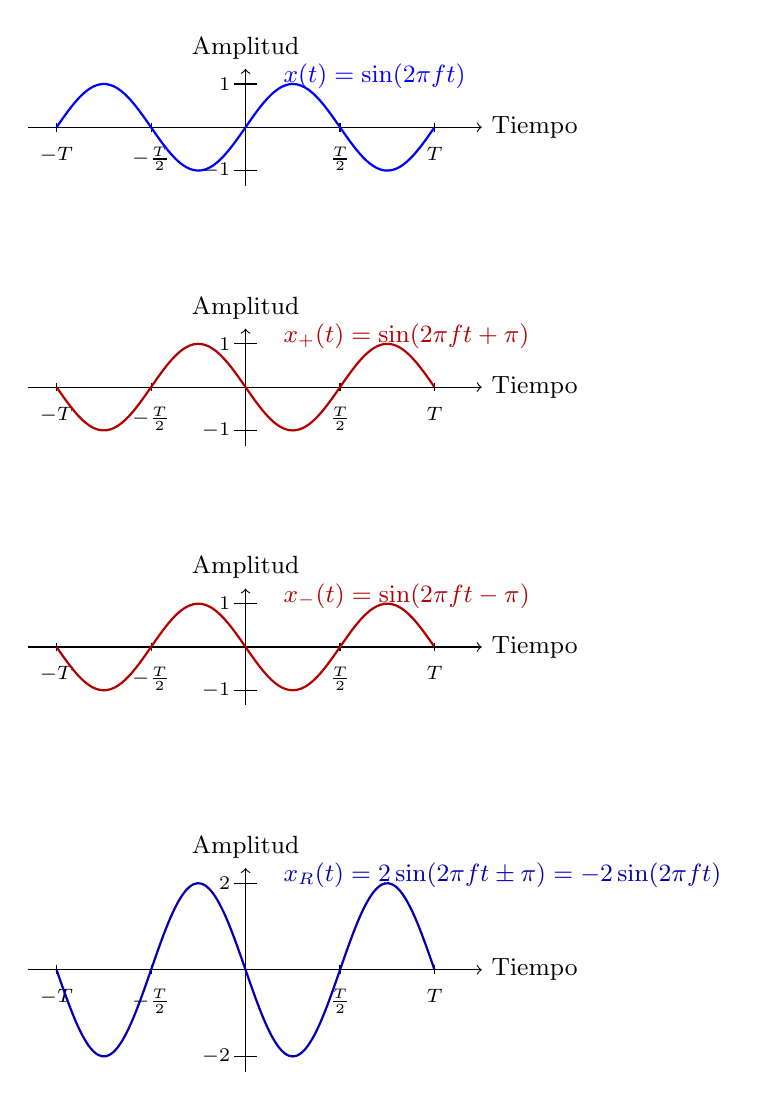
\begin{tikzpicture}[x=2.4cm,y=0.55cm]
    \begin{scope}
      \EjeTiempo{1.35}
      \draw[blue,thick,domain=-1:1,samples=100,smooth]
        plot (\x,{sin(360*\x)});
      \node[blue,anchor=west] at (0.15,1.18) {\small $x(t)=\sin(2\pi ft)$};
      \draw (-0.06,1) -- (0.06,1);
      \draw (-0.06,-1) -- (0.06,-1);
      \node[anchor=east,xshift=-2pt] at (0,1) {\scriptsize $1$};
      \node[anchor=east,xshift=-2pt] at (0,-1) {\scriptsize $-1$};
    \end{scope}

    \begin{scope}[yshift=-3.3cm]
      \EjeTiempo{1.35}
      \draw[red!70!black,thick,domain=-1:1,samples=100,smooth]
        plot (\x,{-sin(360*\x)});
      \node[red!70!black,anchor=west] at (0.15,1.18)
        {\small $x_+(t)=\sin(2\pi ft+\pi)$};
      \draw (-0.06,1) -- (0.06,1);
      \draw (-0.06,-1) -- (0.06,-1);
      \node[anchor=east,xshift=-2pt] at (0,1) {\scriptsize $1$};
      \node[anchor=east,xshift=-2pt] at (0,-1) {\scriptsize $-1$};
    \end{scope}

    \begin{scope}[yshift=-6.6cm]
      \EjeTiempo{1.35}
      \draw[red!70!black,thick,domain=-1:1,samples=100,smooth]
        plot (\x,{-sin(360*\x)});
      \node[red!70!black,anchor=west] at (0.15,1.18)
        {\small $x_-(t)=\sin(2\pi ft-\pi)$};
      \draw (-0.06,1) -- (0.06,1);
      \draw (-0.06,-1) -- (0.06,-1);
      \node[anchor=east,xshift=-2pt] at (0,1) {\scriptsize $1$};
      \node[anchor=east,xshift=-2pt] at (0,-1) {\scriptsize $-1$};
    \end{scope}

    \begin{scope}[yshift=-10.7cm]
      \EjeTiempo{2.35}
      \draw[blue!70!black,thick,domain=-1:1,samples=100,smooth]
        plot (\x,{-2*sin(360*\x)});
      \node[blue!70!black,anchor=west] at (0.15,2.18)
        {\small $x_R(t)=2\sin(2\pi ft\pm\pi)=-2\sin(2\pi ft)$};
      \draw (-0.06,2) -- (0.06,2);
      \draw (-0.06,-2) -- (0.06,-2);
      \node[anchor=east,xshift=-2pt] at (0,2) {\scriptsize $2$};
      \node[anchor=east,xshift=-2pt] at (0,-2) {\scriptsize $-2$};
    \end{scope}
  \end{tikzpicture}
\end{center}

\noindent b).\par\vspace{\baselineskip}
Sean las señales
\[
  x_1(t)=\sin(2\pi ft), \qquad
  x_2(t)=\sin(2\pi ft-\pi)=-\sin(2\pi ft).
\]
El desfase de \(\pi\) hace que \(x_2(t)\) sea la inversa de \(x_1(t)\).
Por ello, para cada instante sus amplitudes se cancelan y la señal resultante
es nula:
\[
  x_R(t)=x_1(t)+x_2(t)
  =\sin(2\pi ft)+\sin(2\pi ft-\pi)=0.
\]

\begin{center}
  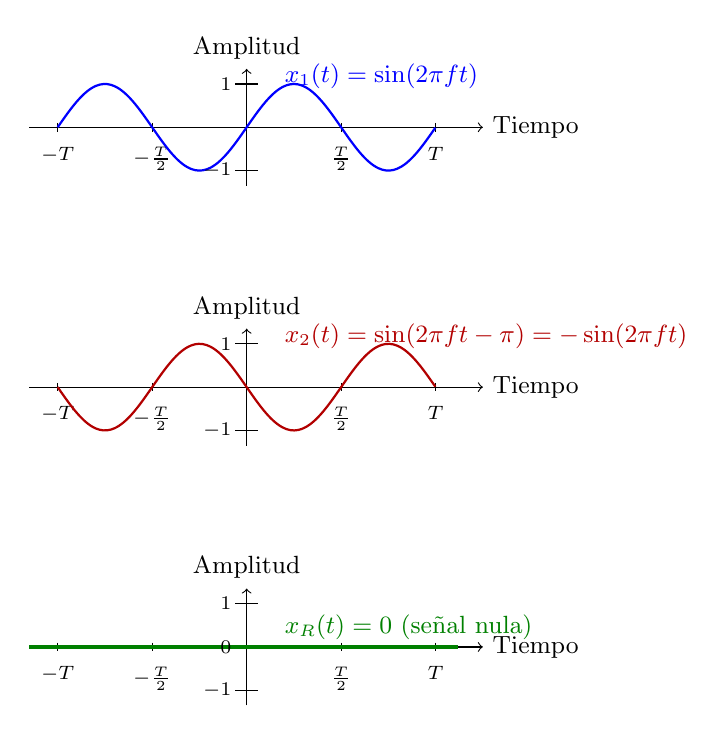
\begin{tikzpicture}[x=2.4cm,y=0.55cm]
    \begin{scope}
      \EjeTiempo{1.35}
      \draw[blue,thick,domain=-1:1,samples=100,smooth]
        plot (\x,{sin(360*\x)});
      \node[blue,anchor=west] at (0.15,1.18)
        {\small $x_1(t)=\sin(2\pi ft)$};
      \draw (-0.06,1) -- (0.06,1);
      \draw (-0.06,-1) -- (0.06,-1);
      \node[anchor=east,xshift=-2pt] at (0,1) {\scriptsize $1$};
      \node[anchor=east,xshift=-2pt] at (0,-1) {\scriptsize $-1$};
    \end{scope}

    \begin{scope}[yshift=-3.3cm]
      \EjeTiempo{1.35}
      \draw[red!70!black,thick,domain=-1:1,samples=100,smooth]
        plot (\x,{-sin(360*\x)});
      \node[red!70!black,anchor=west] at (0.15,1.18)
        {\small $x_2(t)=\sin(2\pi ft-\pi)=-\sin(2\pi ft)$};
      \draw (-0.06,1) -- (0.06,1);
      \draw (-0.06,-1) -- (0.06,-1);
      \node[anchor=east,xshift=-2pt] at (0,1) {\scriptsize $1$};
      \node[anchor=east,xshift=-2pt] at (0,-1) {\scriptsize $-1$};
    \end{scope}

    \begin{scope}[yshift=-6.6cm]
      \EjeTiempo{1.35}
      \draw[green!50!black,very thick] (-1.15,0) -- (1.12,0);
      \node[green!50!black,anchor=west] at (0.15,0.45)
        {\small $x_R(t)=0$ (se\~nal nula)};
      \draw (-0.06,1) -- (0.06,1);
      \draw (-0.06,-1) -- (0.06,-1);
      \node[anchor=east,xshift=-2pt] at (0,1) {\scriptsize $1$};
      \node[anchor=east,xshift=-2pt] at (0,-1) {\scriptsize $-1$};
      \node[anchor=east,xshift=-2pt] at (0,0) {\scriptsize $0$};
    \end{scope}
  \end{tikzpicture}
\end{center}
\noindent\textbf{3.4}\par\vspace{\baselineskip}
\noindent\textbf{3.5}\par\vspace{\baselineskip}
\noindent\textbf{3.6}\par\vspace{\baselineskip}
\noindent\textbf{3.7}\par\vspace{\baselineskip}
\noindent\textbf{3.8}\par\vspace{\baselineskip}
\noindent\textbf{3.9}\par\vspace{\baselineskip}
\noindent\textbf{3.10}\par\vspace{\baselineskip}
\noindent\textbf{3.11}\par\vspace{\baselineskip}
\noindent\textbf{3.12}\par\vspace{\baselineskip}
\noindent\textbf{3.13}\par\vspace{\baselineskip}
\noindent\textbf{3.14}\par\vspace{\baselineskip}
\noindent\textbf{3.15}\par\vspace{\baselineskip}
\noindent\textbf{3.16}\par\vspace{\baselineskip}
\noindent\textbf{3.17}\par\vspace{\baselineskip}
\noindent\textbf{3.18}\par\vspace{\baselineskip}
\noindent\textbf{3.19}\par

Sea un canal con una capacidad de $20\,\text{Mbps}$ y un ancho de banda de
$3\,\text{MHz}$. ¿Cuál es la relación señal-ruido admisible para conseguir
la mencionada capacidad?

Utilizamos la \textbf{Ley de Capacidad de Shannon}:

\[
C = B\log_2(1+\mathrm{SNR})
\]

donde:

\begin{itemize}
    \item $C$: capacidad del canal en bits por segundo (bps).
    \item $B$: ancho de banda en Hz.
    \item $\mathrm{SNR}$: relación señal-ruido en valor adimensional.
\end{itemize}

Datos:

\[
C = 20\,\text{Mbps} = 20\times10^6\,\text{bps}
\]

\[
B = 3\,\text{MHz} = 3\times10^6\,\text{Hz}
\]

Partimos de la expresión de Shannon:

\[
C = B\log_2(1+\mathrm{SNR})
\]

Dividiendo ambos lados por $B$:

\[
\frac{C}{B}
=
\log_2(1+\mathrm{SNR})
\]

Aplicando la función exponencial de base $2$:

\[
1+\mathrm{SNR}
=
2^{\frac{C}{B}}
\]

Por lo tanto:

\[
\mathrm{SNR}
=
2^{\frac{C}{B}}-1
\]

Reemplazando los valores:

\[
\mathrm{SNR}
=
2^{\frac{20\times10^6}{3\times10^6}}-1
\]

\[
\mathrm{SNR}
=
2^{\frac{20}{3}}-1
\]

\[
\mathrm{SNR}
\approx
100.59
\]

Por lo tanto, la relación señal-ruido admisible para conseguir una capacidad
de $20\,\text{Mbps}$ con un ancho de banda de $3\,\text{MHz}$ es:

\[
\boxed{\mathrm{SNR}\approx100.59}
\]
\noindent\textbf{3.20}\par

La onda cuadrada de la Figura 3.7c, con $T=1\,\text{ms}$, se transmite a
través de un filtro paso bajo ideal de ganancia unidad con frecuencia de
corte de $8\,\text{kHz}$.

\textbf{a) Determine la potencia de la señal de salida.}

Primero calculamos la frecuencia fundamental de la onda cuadrada:

\[
f=\frac{1}{T}
\]

Como:

\[
T=1\,\text{ms}=10^{-3}\,\text{s}
\]

entonces:

\[
f=\frac{1}{10^{-3}}
=1000\,\text{Hz}
=1\,\text{kHz}
\]

La onda cuadrada posee únicamente armónicas impares:

\[
k=1,3,5,7,9,\ldots
\]

El filtro tiene una frecuencia de corte:

\[
f_c=8\,\text{kHz}
\]

Por lo tanto, las armónicas que atraviesan el filtro son aquellas que
cumplen:

\[
kf\leq f_c
\]

Como $f=1\,\text{kHz}$:

\[
k(1\,\text{kHz})\leq8\,\text{kHz}
\]

De las armónicas impares, se transmiten:

\[
k=1,3,5,7
\]

La potencia de una onda cuadrada puede expresarse mediante la suma de las
potencias de sus armónicas. Para la señal de la figura:

\[
P_{\text{salida}}
=
\frac{8}{\pi^2}
\left(
\frac{1}{1^2}
+
\frac{1}{3^2}
+
\frac{1}{5^2}
+
\frac{1}{7^2}
\right)
\]

Entonces:

\[
P_{\text{salida}}
=
\frac{8}{\pi^2}
\left(
1+\frac{1}{9}+\frac{1}{25}+\frac{1}{49}
\right)
\]

\[
P_{\text{salida}}
\approx0.95\,\text{W}
\]

Por lo tanto:

\[
\boxed{P_{\text{salida}}\approx0.95\,\text{W}}
\]

\bigskip

\textbf{b) Suponiendo que a la entrada del filtro hay un ruido térmico con
$N_0=0.1\,\mu\text{W}/\text{Hz}$, encuentre la relación señal-ruido en dB
a la salida.}

La densidad espectral de potencia del ruido es:

\[
N_0=0.1\,\mu\text{W}/\text{Hz}
\]

El ancho de banda que deja pasar el filtro paso bajo ideal es:

\[
B=8\,\text{kHz}=8000\,\text{Hz}
\]

La potencia total del ruido a la salida es:

\[
P_n=N_0B
\]

Reemplazando:

\[
P_n=
(0.1\,\mu\text{W}/\text{Hz})(8000\,\text{Hz})
\]

\[
P_n=800\,\mu\text{W}
\]

Como:

\[
800\,\mu\text{W}=0.0008\,\text{W}
\]

la relación señal-ruido es:

\[
\mathrm{SNR}
=
\frac{P_{\text{señal}}}{P_n}
\]

\[
\mathrm{SNR}
=
\frac{0.95}{0.0008}
\]

\[
\mathrm{SNR}=1187.5
\]

Para expresar la relación señal-ruido en decibelios:

\[
\mathrm{SNR}_{dB}
=
10\log_{10}(\mathrm{SNR})
\]

Por lo tanto:

\[
\mathrm{SNR}_{dB}
=
10\log_{10}(1187.5)
\]

\[
\mathrm{SNR}_{dB}
\approx30.74\,\text{dB}
\]

Por lo tanto, la relación señal-ruido a la salida es:

\[
\boxed{\mathrm{SNR}_{dB}\approx30.74\,\text{dB}}
\]
\section*{d)- Modulacion de AM en Python}

\end{document}
